\documentclass{article}

\usepackage{physics} % Handy shortcuts like \pdv, \dd and much more
\usepackage{geometry} % smaller margins, can be adjusted if given arguments
\usepackage{siunitx} % the \si environment for units
\usepackage{mathtools} % The dcases environment, prettier than just cases, imports amsmath
\usepackage{tikz} % For drawing picures
\usepackage{wrapfig} % Wrapping text around figures
\usepackage{bbold}


\title{Exercise 7 solutions - TFY4345 Classical Mechanics}
\date{2020}

\begin{document}
    \maketitle
    \section{Inertia tensor}
        (SIDEREFFERANSE)\\
        The inertia tensor of a solid object $V$ with the mass density $\rho(\vec r)$ is defined as
        \begin{equation*}
            I_{ij} = \int_V \rho(\vec{r}) \big(\delta_{ij} r^2 - x_ix_j) \dd V.
        \end{equation*}
        We assume the slab is so thin that the $z$-direction can be neglected, and that it has a constant mass density $\rho = M / ab$. The integral then becomes.
        \begin{equation*}
            I_{ij} = \frac{M}{ab} \int_0^a \dd x \int_0^b \dd y ( r^2 - x_ix_j).
        \end{equation*}
        We see that $I_{ij} = I_{ji}$, so inserting $x_1 = x, \, x_2 = y, \, x_3 = z, \, r = \sqrt{x^2 + y^2 + z^2}, \, z = 0$, the integral needed are
        \begin{equation*}
            \begin{dcases}
                I_{1 1} = \frac{M}{ab} \int_0^a \dd x \int_0^b \dd y (y^2 + z^2) = \frac{1}{3}Mb^2\\
                I_{1 2} = \frac{M}{ab} \int_0^a \dd x \int_0^b \dd y (-xy) -\frac{1}{4}M ab\\
                I_{1 3} = \frac{M}{ab} \int_0^a \dd x \int_0^b \dd y (-xz) = 0\\
                I_{2 2} = \frac{M}{ab} \int_0^a \dd x \int_0^b \dd y (x^2 + z^2) = \frac{1}{3}Ma^2\\
                I_{2 3} = \frac{M}{ab} \int_0^a \dd x \int_0^b \dd y (-yz) = 0\\
                I_{3 3} = \frac{M}{ab} \int_0^a \dd x \int_0^b \dd y (x^2 + y^2) = \frac{1}{3}M(a^2 + b^2)\\
            \end{dcases}    
        \end{equation*}
        This gives the inertia tensor
        \begin{equation*}
            I = \begin{pmatrix}
                I_{11} & I_{12} & I_{13} \\
                I_{21} & I_{22} & I_{23} \\
                I_{31} & I_{32} & I_{33} \\
            \end{pmatrix}
            =
            \begin{pmatrix}
                \frac{1}{3}Mb^2 & -\frac{1}{4}Mab & 0 \\
                -\frac{1}{4}Mab & \frac{1}{3}Ma^2 & 0 \\
                0 & 0 & \frac{1}{3}M(a^2 + b^2)   \\
            \end{pmatrix}
        \end{equation*}
        b) Let $a = b$, and define $\beta = 1/3 Ma^2$. Then, 
        \begin{equation*}
            I =
            \begin{pmatrix}
                \frac{1}{3}Mb^2 & -\frac{1}{4}Mab & 0 \\
                -\frac{1}{4}Mab & \frac{1}{3}Ma^2 & 0 \\
                0 & 0 & \frac{1}{3}M(a^2 + b^2)   \\
            \end{pmatrix}
            = \beta
            \begin{pmatrix}
            1 & -\frac{3}{4}  & 0 \\
            -\frac{3}{4}  & 1 & 0 \\
            0 & 0 & 2  \\
            \end{pmatrix}
        \end{equation*}
        The principal axes are the coordinate axis in which the inertia tensor is diagonal, and the corresponding values for the inertia tensor are the principal moments of inertia. Remembering our linear algebra we thus need to find the eigenvalues of the inertia tensor. The characteristic polynomial is
        \begin{align*}
            |I - \lambda \mathbb{1} | = 
            \begin{vmatrix}
                \beta - \lambda & -\frac{3}{4} \beta  & 0 \\
                -\frac{3}{4}\beta  & \beta - \lambda & 0 \\
                0 & 0 & 2\beta - \lambda  \\
            \end{vmatrix}
            = (2\beta - \lambda)\bigg((\beta - \lambda)^2 - \frac{9}{16} \beta^2\bigg) = 0
        \end{align*}
        This has the solution $\lambda = 2\beta$, or
        \begin{equation*}
            \lambda^2 - 2 \beta \lambda + \bigg(\beta^2 - \frac{9}{16} \beta^2 \bigg) = 0 
            \implies \lambda = \frac{1}{2}\bigg( 2\beta \pm \sqrt{(2 \beta)^2 - 4 \bigg(\beta^2 - \frac{9}{16} \beta^2 \bigg)} \bigg) 
            = \beta \bigg(1 \pm \frac{3}{4}\bigg).
        \end{equation*}
        This leaves us with the diagonalized inertia tensor, with the principal moments of inertia
        \begin{equation*}
            I' = 
            \begin{pmatrix}
                I'_{11} & 0 & 0 \\
                0 & I'_{22} & 0 \\
                0 & 0 & I'_{33} \\
            \end{pmatrix}
            = \beta
            \begin{pmatrix}
                2 & 0 & 0 \\
                0 & \frac{1}{4} & 0 \\
                0 & 0 & \frac{7}{4} \\
            \end{pmatrix}
            = Ma^2
            \begin{pmatrix}
                \frac{1}{12} & 0 & 0 \\
                0 & \frac{7}{12} & 0  \\
                0 & 0 & \frac{2}{3} \\
            \end{pmatrix}
        \end{equation*}
        This inertia tensor corresponds to rotation around a different set axes, the principal axes $\boldsymbol{\omega}^{(1)}, \boldsymbol{\omega}^{(2)}, \boldsymbol{\omega}^{(2)}$, than the original, which corresponds to rotation around the $xyz$-axes. The defining feature of the principal axis is that
        \begin{equation*}
            I \boldsymbol{\omega^{(i)}} = I_i' \boldsymbol{\omega^{(i)}},
        \end{equation*}
        so we need to find the normalized eigenvalues of $I$. The equations for these are
        \begin{equation*}
            I \boldsymbol{\omega^{(i)}} = \beta
            \begin{pmatrix}
                1 & -\frac{3}{4}  & 0 \\
                -\frac{3}{4}  & 1 & 0 \\
                0 & 0 & 2  \\
            \end{pmatrix}
            \begin{pmatrix*}
                \omega^{(i)}_1 \\
                \omega^{(i)}_2 \\
                \omega^{(i)}_3 \\
            \end{pmatrix*}
            = 
            I'_{ii}
            \begin{pmatrix*}
                \omega^{(i)}_1 \\
                \omega^{(i)}_2 \\
                \omega^{(i)}_3 \\
            \end{pmatrix*}
        \implies
        \begin{dcases*}
            \beta (\omega^{(i)}_1 - \frac{3}{4} \omega^{(i)}_2) = I_{ii}\omega^{(i)}_1 \\
            \beta (- \frac{3}{4} \omega^{(i)}_1 + \omega^{(i)}_1) = I_{ii}'\omega^{(i)}_2 \\
            2 \beta \omega^{(i)}_3 = I_{ii}' \omega^{(i)}_3
        \end{dcases*}
        \end{equation*}

        We can immediately see that $i = 3$ gives
        \begin{equation*}
            \boldsymbol{\omega}^{(3)} = 
            \begin{pmatrix}
                0 \\
                0 \\
                1 \\
            \end{pmatrix}
            \implies I \boldsymbol{\omega}^{(3)} = I_{33}' \boldsymbol{\omega}^{(3)}  = \frac{2}{3} Ma^2 \boldsymbol{\omega}^{(3)} 
        \end{equation*}
        $i= 1, \, I_{11}' = \frac{1}{4}\beta$ gives
        \begin{equation*}
            \begin{dcases*}
                \beta (\omega^{(i)}_1 - \frac{3}{4} \omega^{(i)}_2) = \frac{1}{4}\beta\omega^{(i)}_1 \\
                \beta (- \frac{3}{4} \omega^{(i)}_1 + \omega^{(i)}_1) = \frac{1}{4}\beta \omega^{(i)}_2 \\
                2 \beta \omega^{(i)}_3 = \frac{1}{4}\beta \omega^{(i)}_3
            \end{dcases*}
            \implies 
            \boldsymbol{\omega}^{(3)} = \frac{1}{\sqrt{2}}
                \begin{pmatrix}
                    1 \\
                    1 \\
                    0 \\
                \end{pmatrix}
        \end{equation*}
        while $i = 2, \, I_{22}' = \frac{7}{4}\beta$ gives
        \begin{equation*}
            \begin{dcases*}
                \beta (\omega^{(i)}_1 - \frac{3}{4} \omega^{(i)}_2) = \frac{7}{4}\beta\omega^{(i)}_1 \\
                \beta (- \frac{3}{4} \omega^{(i)}_1 + \omega^{(i)}_1) = \frac{7}{4}\beta \omega^{(i)}_2 \\
                2 \beta \omega^{(i)}_3 = \frac{1}{4}\beta \omega^{(i)}_3
            \end{dcases*}
            \implies 
            \boldsymbol{\omega}^{(3)} = \frac{1}{\sqrt{2}}
                \begin{pmatrix}
                    -1 \\
                    1 \\
                    0 \\
                \end{pmatrix}
        \end{equation*}
    
    \section{Rotated tilted slab}
        a) \\ \\  
        Given the moment of inertia around the principal axes
        \begin{equation*}
            I = M
            \begin{pmatrix}
                \frac{1}{12} a^2& 0 & 0 \\
                0 & \frac{1}{12} b^2 & 0 \\
                0 & 0 & \frac{1}{12} (a^2 + b^2)\\
            \end{pmatrix}
        \end{equation*}
        the angular momentum is given by
        \begin{equation*}
            \mathbf{L} = I \mathbf{\omega} = \sum_i  I_i \omega_i  \mathbf{e}_i.
        \end{equation*}
        By looking at the illustration, we can express
        \begin{equation*}
            \sin(\theta) = \frac{b}{\sqrt{a^2 + b^2}}, \quad \sin(\theta) = \frac{a}{\sqrt{a^2 + b^2}},
        \end{equation*}
        The the angular velocity vector in the principal axis system is then
        \begin{equation*}
            \boldsymbol{\omega} = \sum_i \omega_i \mathbf{e}_i = \omega (-\sin(\theta) \mathbf{e}_1 + \cos(\theta) \mathbf{e}_2) = \frac{1}{12}\frac{\omega}{\sqrt{a^2 + b^2}}(-b \mathbf{e}_1 + a \mathbf{e}_2)
        \end{equation*} 
        The angular momentum vector is therefore
        \begin{equation*}
            \mathbf{L} = \frac{1}{12} M \omega(-a^2\sin(\theta) \mathbf{e}_1 + b^2\cos(\theta) \mathbf{e}_2)
        \end{equation*}
        Thus, in general, the angular momentum and velocity vector are not parallel. 
        which gives
        \begin{equation*}
            \mathbf{L} = \frac{1}{12}\frac{M \omega}{\sqrt{a^2 + b^2}}(-a^2b \mathbf{e}_1 + b^2a \mathbf{e}_2)
        \end{equation*} 
        \\ \\
        b) \\ \\
        The angle between two vectors is given by the dot product,
        \begin{equation*}
            \boldsymbol \omega \cdot \mathbf{L} = \omega L \cos(\alpha) \implies \alpha = \arccos\bigg( \frac{\boldsymbol \omega \cdot \mathbf{L}}{\omega L}\bigg).
        \end{equation*}
        These quantities are given by
        \begin{align*}
            &\boldsymbol \omega \cdot \mathbf{L}  = \frac{1}{12} M \bigg( \frac{\omega}{\sqrt{a^2 + b^2}}\bigg)^2 (a^2b^2 + a^2b^2) = \frac{1}{12}\frac{2M}{a^2+ b^2} ( ab\omega)^2 \\
            &L^2 = \mathbf{L} \cdot \mathbf{L} = \bigg(\frac{M \omega}{\sqrt{a^2 + b^2}}\bigg)^2 ((a^2b)^2 + (b^2a)^2) = \bigg( \frac{1}{12}M \omega\bigg)^2 \bigg( a^2b^2\frac{a^2 + b^2}{a^2 + b^2}\bigg) = \bigg( \frac{1}{12} abM\omega \bigg)^2 \\
        \implies & \alpha = \arccos \bigg( 
            \frac{1}{12}\frac{2M}{a^2+ b^2} ( ab\omega)^2 \bigg/ \frac{1}{12} abM\omega^2 \bigg)
            = \arccos\bigg(\frac{2ab}{a^2 + b^2}\bigg).
        \end{align*}
        For example, with $b=1, a=2$, we get $\alpha = 36.9^\circ, \theta = 26.6^\circ$.
        \\ \\
        c) 
        \\ \\
        The rotational kinetic energy is given by 
        \begin{equation*}
            T_{rot} = \frac{1}{2} \boldsymbol \omega \cdot \mathbf{L} = \frac{1}{12}\frac{( ab)^2}{a^2+ b^2} M \omega^2.
    \end{equation*}

    \section{Cone rolling on a plane}
        \begin{wrapfigure}{r}{0.35\textwidth}
            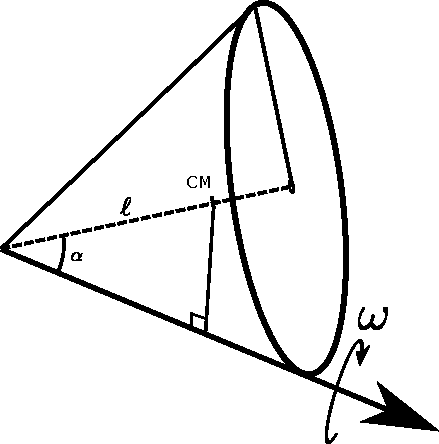
\includegraphics[width=0.35\textwidth]{figures/exercise_7_3_cone2.pdf}
        \end{wrapfigure}
        a) \\ \\
        The axis $x_3$ is always straight above the line $OA$, and has therefore the same angular velocity, $\dot \phi$. Observing the figure, we see that the center of mass is at a distance $\ell \cos(\alpha)$ from the $z$-axis, so the center of mass velocity is
        \begin{equation*}
            V_{CM} = \ell \cos(\alpha) \dot \phi
        \end{equation*} 

        b) \\ \\
        The fact that the contact point of the cone and the plane is just a line, and that it rotates without slipping, means that at every instant it rotates just as it would have if were just rotating around a line. However, in the next instant, the line of contact has moved, so it has an instantaneous axis of rotation parallel to the line $OA$. We can find the angular velocity using how the center-of-mass moves with respect to $OA$. The point on the line $OA$ below the center-of-mass is at a length $\ell \sin(\alpha)$ from the $z$-axis, so the angular velocity of the cone is

        c) \\ \\        
        \begin{equation*}
            \omega = \frac{V_{cm}}{\ell \sin(\alpha)} = \frac{\cos(\alpha)}{\sin(\alpha)} \dot \phi
        \end{equation*}  
        The figure shows two of the principal axis, the third one is into the page, perpendicular to $x_1$ and $x_2$. The moment of inertia tensor in this can be expressed in this system as 
        \newpage % Figure must be placed on the page where it appears
        \begin{wrapfigure}{R}{0.3\textwidth}         
            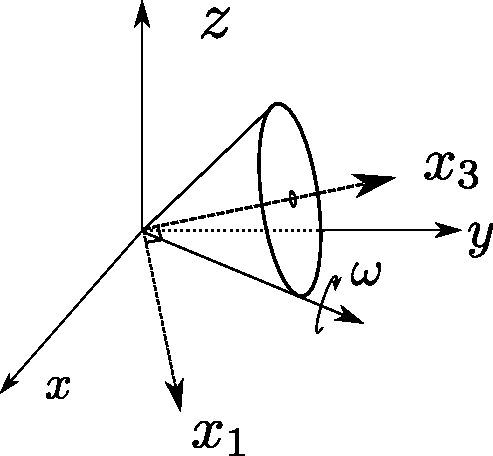
\includegraphics[width=0.3\textwidth]{figures/exercise_7_3_cone3.pdf}
        \end{wrapfigure}
        \begin{align*}
            \boldsymbol{\omega} = \sum_i \omega_i \mathbf{e}_i,
        \end{align*}
        and due to our choice of $x_2$, $\omega_2 = 0$. The two other components are then
        \begin{align*}
            &\omega_1 = \omega \sin(\alpha) =  \cos(\alpha) \dot \phi,  \\
            &\omega_3 = \omega \cos(\alpha) =  \frac{\cos^2(\alpha)}{\sin(\alpha)} \dot \phi
        \end{align*}
        d) \\ \\
        The kinetic energy of a rotating object is
        \begin{align*}
            &\frac{1}{2} \boldsymbol{\omega}^T I \boldsymbol{\omega} = \frac{3}{20} M
            \begin{pmatrix*}
                \omega_1 &
                0&
                \omega_3
            \end{pmatrix*}
            \begin{pmatrix}
                R^2 + 4H^2& 0 & 0 \\
                0 & R^2 + 4H^2& 0 \\
                0 & 0 & 2R^2\\
            \end{pmatrix}
            \begin{pmatrix*}
                \omega_1 \\
                0 \\
                \omega_3
            \end{pmatrix*}
            = \frac{3}{20} M \bigg(\omega_1^2 (R^2 + 4H^2) + 2\omega_3^2R^2\bigg) \\
            = &\frac{3}{40} M \dot \phi^2 \bigg(\cos^2(\alpha)\bigg(\bigg[\frac{\sin(\alpha)}{\cos(\alpha)}\bigg]^2H^2 + 4H^2\bigg) + 2\frac{\cos^4(\alpha)}{\sin^2(\alpha)}\bigg[\frac{\sin(\alpha)}{\cos(\alpha)}\bigg]^2H^2 \bigg) \\
            = &\frac{3}{40} M \dot \phi^2 H^2 \bigg(\sin^2(\alpha) + 4\cos^2(\alpha)+ 2 \cos^2(\alpha)\bigg) = \frac{3}{40} M \dot \phi^2 H^2 \bigg(1 + 5\cos^2(\alpha)\bigg)
        \end{align*}
        where we use that $R\cos(\alpha) =  H \sin(\alpha)$.
\end{document}
